\chapter{Numbers 13}

\begin{figure}
  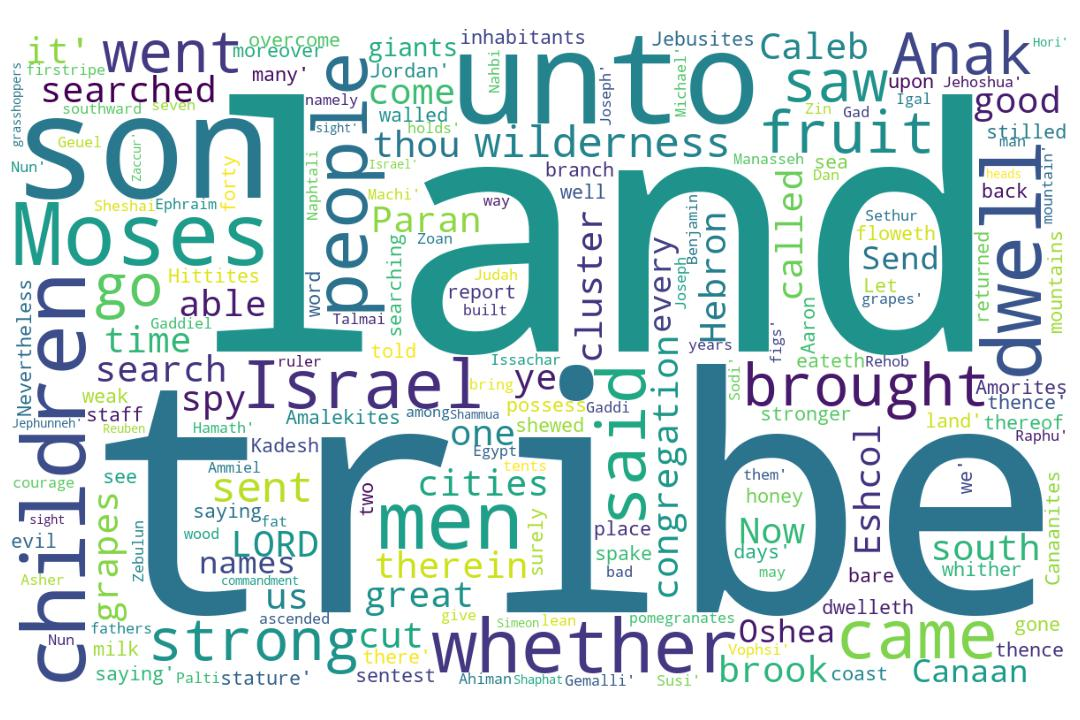
\includegraphics[width=\linewidth]{04OT-Numbers/Numbers13-WordCloud.jpg}
  \caption{Numbers 13 Word Cloud}
  \label{fig:Numbers 13 word Cloud}
\end{figure}



\marginpar{\scriptsize \centering \fcolorbox{bone}{lime}{\textbf{A 40-YEAR MISTAKE}}\\ (Numbers 13:1-33) \begin{compactenum}[I.][8]
    \item An \textbf{Inspection Tour} \index[scripture]{Numbers!Num 13:17}(Num 13:17) 
    \item An \textbf{Important Test} \index[scripture]{Numbers!Num 13:25}(Num 13:25) 
    \item \textbf{Impenetrable Towns} \index[scripture]{Numbers!Num 13:28}(Num 13:28) 
    \item \textbf{Insolent Transgressors} \index[scripture]{Numbers!Num 13:31}(Num 13:31) 
    \item People \textbf{Impressive \& Tall} \index[scripture]{Numbers!Num 13:32, 33}(Num 13:32, 33) 
    \item As \textbf{Insignificant Tourists} \index[scripture]{Numbers!Num 13:33}(Num 13:33) 
    \item An \textbf{Instructive Time} %\index[scripture]{Numbers!Numbers 13:17}(Numbers 13:17) 
\end{compactenum}}


\marginpar{\scriptsize \centering \fcolorbox{bone}{yellow}{\textbf{REBELLION AT KADESH}}\\ (Numbers 13:1-33) \begin{compactenum}[I.][8]
   \item The \textbf{Sending}  \index[scripture]{Numbers!Num 13:01}    (Num 13:1) 
   \item The \textbf{Search} \index[scripture]{Numbers!Num 13:01}  \index[scripture]{Numbers!Num 13:21}  \index[scripture]{Numbers!Num 13:25}\index[scripture]{Numbers!Num 13:32}  (Num 13:1, 21, 25, 32) 
   \item The \textbf{Sons}  \index[scripture]{Numbers!Num 13:04--15}    (Num 13:4--15) 
    \item The \textbf{Strength} of the Enemy \index[scripture]{Numbers!Num 13:18}\index[scripture]{Numbers!Num 13:28} \index[scripture]{Numbers!Num 13:31}  (Num 13:18, 28, 31) 
   \item The \textbf{Stature}  \index[scripture]{Numbers!Num 13:32}    (Num 13:32) 
   \item The \textbf{Sight}  of the Spies \index[scripture]{Numbers!Num 13:33}    (Num 13:33) 
  \item The \textbf{Significance} of Unbelief %\index[scripture]{Numbers!Num 13:01}    (Numbers 13:1) 
\end{compactenum}}

\marginpar{\scriptsize \centering \fcolorbox{bone}{black}{\textbf{\textcolor[cmyk]{0,0,0,0}{THE SPIES}}}\\ (Numbers 13:1-33) 
 \begin{compactenum}[I.][8]
   \item \textbf{Required} for the Mission \index[scripture]{Numbers!Num 13:02}    (Num 13:2) 
   \item \textbf{Represented} the Tribes \index[scripture]{Numbers!Num 13:02}    (Num 13:2) 
   \item \textbf{Recounted} the Enemies\index[scripture]{Numbers!Num 13:27--28}    (Num 13:27--28)
   \item \textbf{Rebelled}  \index[scripture]{Numbers!Num 13:31}    (Num 13:31)
   \item \textbf{Disregarded} the LORD \index[scripture]{Numbers!Num 13:31}    (Num 13:31)
   \item \textbf{Ruined} the chances to Enter the Land  ... for 40 years, and the death of over 600,000 men plus women and children and the strangers who were with them
   \item Didn't \textbf{Recognize} what they had with them
\end{compactenum}}

\marginpar{\scriptsize \centering \fcolorbox{bone}{blue}{\textcolor{white}{\textbf{THE SPIES DID NOT SEE}}}\\ (Numbers 13:1-33) 
 \begin{compactenum}[I.][8]
   \item The \textbf{Goodness} that Awaited \index[scripture]{Numbers!Num 13:32}    (Numbers 13:32) 
   \item The \textbf{Giants} Annihilated
   \item A \textbf{God} who is Awesome -- Bigger than the Giants 
   \item The \textbf{Grief} After their rebellion -- a defeat in the next chapter, a 40-year wait
   \item The \textbf{Guidance} that was Available
   \item  \textbf{Great} Victories Ahead
   \item The \textbf{Glory} of God Above all Else
\end{compactenum}}


\footnote{\textcolor[cmyk]{0.99998,1,0,0}{\hyperlink{TOC}{Return to end of Table of Contents.}}}\footnote{\href{https://audiobible.com/bible/numbers_13.html}{\textcolor[cmyk]{0.99998,1,0,0}{Numbers 13 Audio}}}\textcolor[cmyk]{0.99998,1,0,0}{And the LORD spake unto Moses, saying,}
[2] \textcolor[cmyk]{0.99998,1,0,0}{Send thou men, that they may search the land of Canaan, which I give unto the children of Israel: of every tribe of their fathers shall ye send a man, every one a ruler among them.}
[3] \textcolor[cmyk]{0.99998,1,0,0}{And Moses by the commandment of the LORD sent them from the wilderness of Paran: all those men \emph{were} heads of the children of Israel.}
[4] \textcolor[cmyk]{0.99998,1,0,0}{And these \emph{were} their names: of \fcolorbox{bone}{bone}{the tribe} of Reuben, Shammua the \fcolorbox{bone}{bone}{son} of Zaccur.}
[5] \textcolor[cmyk]{0.99998,1,0,0}{Of \fcolorbox{bone}{bone}{the tribe} of Simeon, Shaphat the \fcolorbox{bone}{bone}{son} of Hori.}
[6] \textcolor[cmyk]{0.99998,1,0,0}{Of \fcolorbox{bone}{bone}{the tribe} of Judah, Caleb the \fcolorbox{bone}{bone}{son} of Jephunneh.}
[7] \textcolor[cmyk]{0.99998,1,0,0}{Of \fcolorbox{bone}{bone}{the tribe} of Issachar, Igal the \fcolorbox{bone}{bone}{son} of Joseph.}
[8] \textcolor[cmyk]{0.99998,1,0,0}{Of \fcolorbox{bone}{bone}{the tribe} of Ephraim, Oshea the \fcolorbox{bone}{bone}{son} of Nun.}
[9] \textcolor[cmyk]{0.99998,1,0,0}{Of \fcolorbox{bone}{bone}{the tribe} of Benjamin, Palti the \fcolorbox{bone}{bone}{son} of Raphu.}
[10] \textcolor[cmyk]{0.99998,1,0,0}{Of \fcolorbox{bone}{bone}{the tribe} of Zebulun, Gaddiel the \fcolorbox{bone}{bone}{son} of Sodi.}
[11] \textcolor[cmyk]{0.99998,1,0,0}{Of \fcolorbox{bone}{bone}{the tribe} of Joseph, \emph{namely}, of \fcolorbox{bone}{bone}{the tribe} of Manasseh, Gaddi the \fcolorbox{bone}{bone}{son} of Susi.}
[12] \textcolor[cmyk]{0.99998,1,0,0}{Of \fcolorbox{bone}{bone}{the tribe} of Dan, Ammiel the \fcolorbox{bone}{bone}{son} of Gemalli.}
[13] \textcolor[cmyk]{0.99998,1,0,0}{Of \fcolorbox{bone}{bone}{the tribe} of Asher, Sethur the \fcolorbox{bone}{bone}{son} of Michael.}
[14] \textcolor[cmyk]{0.99998,1,0,0}{Of \fcolorbox{bone}{bone}{the tribe} of Naphtali, Nahbi the \fcolorbox{bone}{bone}{son} of Vophsi.}
[15] \textcolor[cmyk]{0.99998,1,0,0}{Of \fcolorbox{bone}{bone}{the tribe} of Gad, Geuel the \fcolorbox{bone}{bone}{son} of Machi.}
[16] \textcolor[cmyk]{0.99998,1,0,0}{These \emph{are} the names of the men which Moses sent to spy out the land. And Moses called Oshea the \fcolorbox{bone}{bone}{son} of Nun Jehoshua.}\\
\\
\P \textcolor[cmyk]{0.99998,1,0,0}{And Moses sent them to spy out the land of Canaan, and said unto them, Get you up this \emph{way} southward, and go up into the mountain:}
[18] \textcolor[cmyk]{0.99998,1,0,0}{And see the land, what it \emph{is}; and the people that dwelleth therein, whether they \emph{be} strong or weak, few or many;}
[19] \textcolor[cmyk]{0.99998,1,0,0}{And what the land \emph{is} that they dwell in, whether it \emph{be} good or bad; and what cities \emph{they} \emph{be} that they dwell in, whether in tents, or in strong holds;}
[20] \textcolor[cmyk]{0.99998,1,0,0}{And what the land \emph{is}, whether it \emph{be} fat or lean, whether there be wood therein, or not. And be ye of good courage, and bring of the fruit of the land. Now the time \emph{was} the time of the firstripe grapes.}\\
\\
\P \textcolor[cmyk]{0.99998,1,0,0}{So they went up, and searched the land from the wilderness of Zin unto Rehob, as men come to Hamath.}
[22] \textcolor[cmyk]{0.99998,1,0,0}{And they ascended by the south, and came unto Hebron; where Ahiman, Sheshai, and Talmai, the children of Anak, \emph{were}. (Now Hebron was built seven years before Zoan in Egypt.)}
[23] \textcolor[cmyk]{0.99998,1,0,0}{And they came unto the brook of Eshcol, and cut down from thence a branch with one cluster of grapes, and they bare it between two upon a staff; and \emph{they} \emph{brought} of the pomegranates, and of the figs.}
[24] \textcolor[cmyk]{0.99998,1,0,0}{The place was called the brook Eshcol, because of the cluster of grapes which the children of Israel cut down from thence.}
[25] \textcolor[cmyk]{0.99998,1,0,0}{And they returned from searching of the land after forty days.}\\
\\
\P \textcolor[cmyk]{0.99998,1,0,0}{And they went and came to Moses, and to Aaron, and to all the congregation of the children of Israel, unto the wilderness of Paran, to Kadesh; and brought back word unto them, and unto all the congregation, and shewed them the fruit of the land.}
[27] \textcolor[cmyk]{0.99998,1,0,0}{And they told him, and said, We came unto the land whither thou sentest us, and surely it floweth with milk and honey; and this \emph{is} the fruit of it.}
[28] \textcolor[cmyk]{0.99998,1,0,0}{Nevertheless the people \emph{be} strong that dwell in the land, and the cities \emph{are} walled, \emph{and} very great: and moreover we saw the children of Anak there.}
[29] \textcolor[cmyk]{0.99998,1,0,0}{The Amalekites dwell in the land of the south: and the Hittites, and the Jebusites, and the Amorites, dwell in the mountains: and the Canaanites dwell by the sea, and by the coast of Jordan.}
[30] \textcolor[cmyk]{0.99998,1,0,0}{And Caleb stilled the people before Moses, and said, Let us go up at once, and possess it; for we are well able to overcome it.}
[31] \textcolor[cmyk]{0.99998,1,0,0}{But the men that went up with him said, We be not able to go up against the people; for they \emph{are} stronger than we.}
[32] \textcolor[cmyk]{0.99998,1,0,0}{And they brought up an evil report of the land which they had searched unto the children of Israel, saying, The land, through which we have gone to search it, \emph{is} a land that eateth up the inhabitants thereof; and all the people that we saw in it \emph{are} men of a great stature.}
[33] \textcolor[cmyk]{0.99998,1,0,0}{And there we saw the giants, the sons of Anak, \emph{which} \emph{come} of the giants: and we were in our own sight as grasshoppers, and so we were in their sight.}

